%---------------------------------------------------------------
\chapter{Nasazení}
%---------------------------------------------------------------

\begin{chapterabstract}
    V této kapitole popíšu proces nasazení serveru na virtuální stroj a nasazení aplikace do obchodu pro iOS/macOS aplikace App Store.
\end{chapterabstract}

\section{Server}

Pro to, aby mohla aplikace s REST API komunikovat, musí být REST API veřejně přístupné, proto jsem se rozhodl jej nasadit na virtuální stroj. U společnosti Hicoria \cite{hicoria} pronajímám virtuální stroj s operačním systémem Debian, 1 GB RAM a 20 GB SSD disku za cenu přibližně 650 Kč ročně. Na tomto stroji již hostuji své webové stránky a dohodl jsem se s náboženskými shromážděními, že tento stroj poskytnu i pro účely nasazení serveru poskytujícího podpůrné REST API.

\begin{figure}[H]
    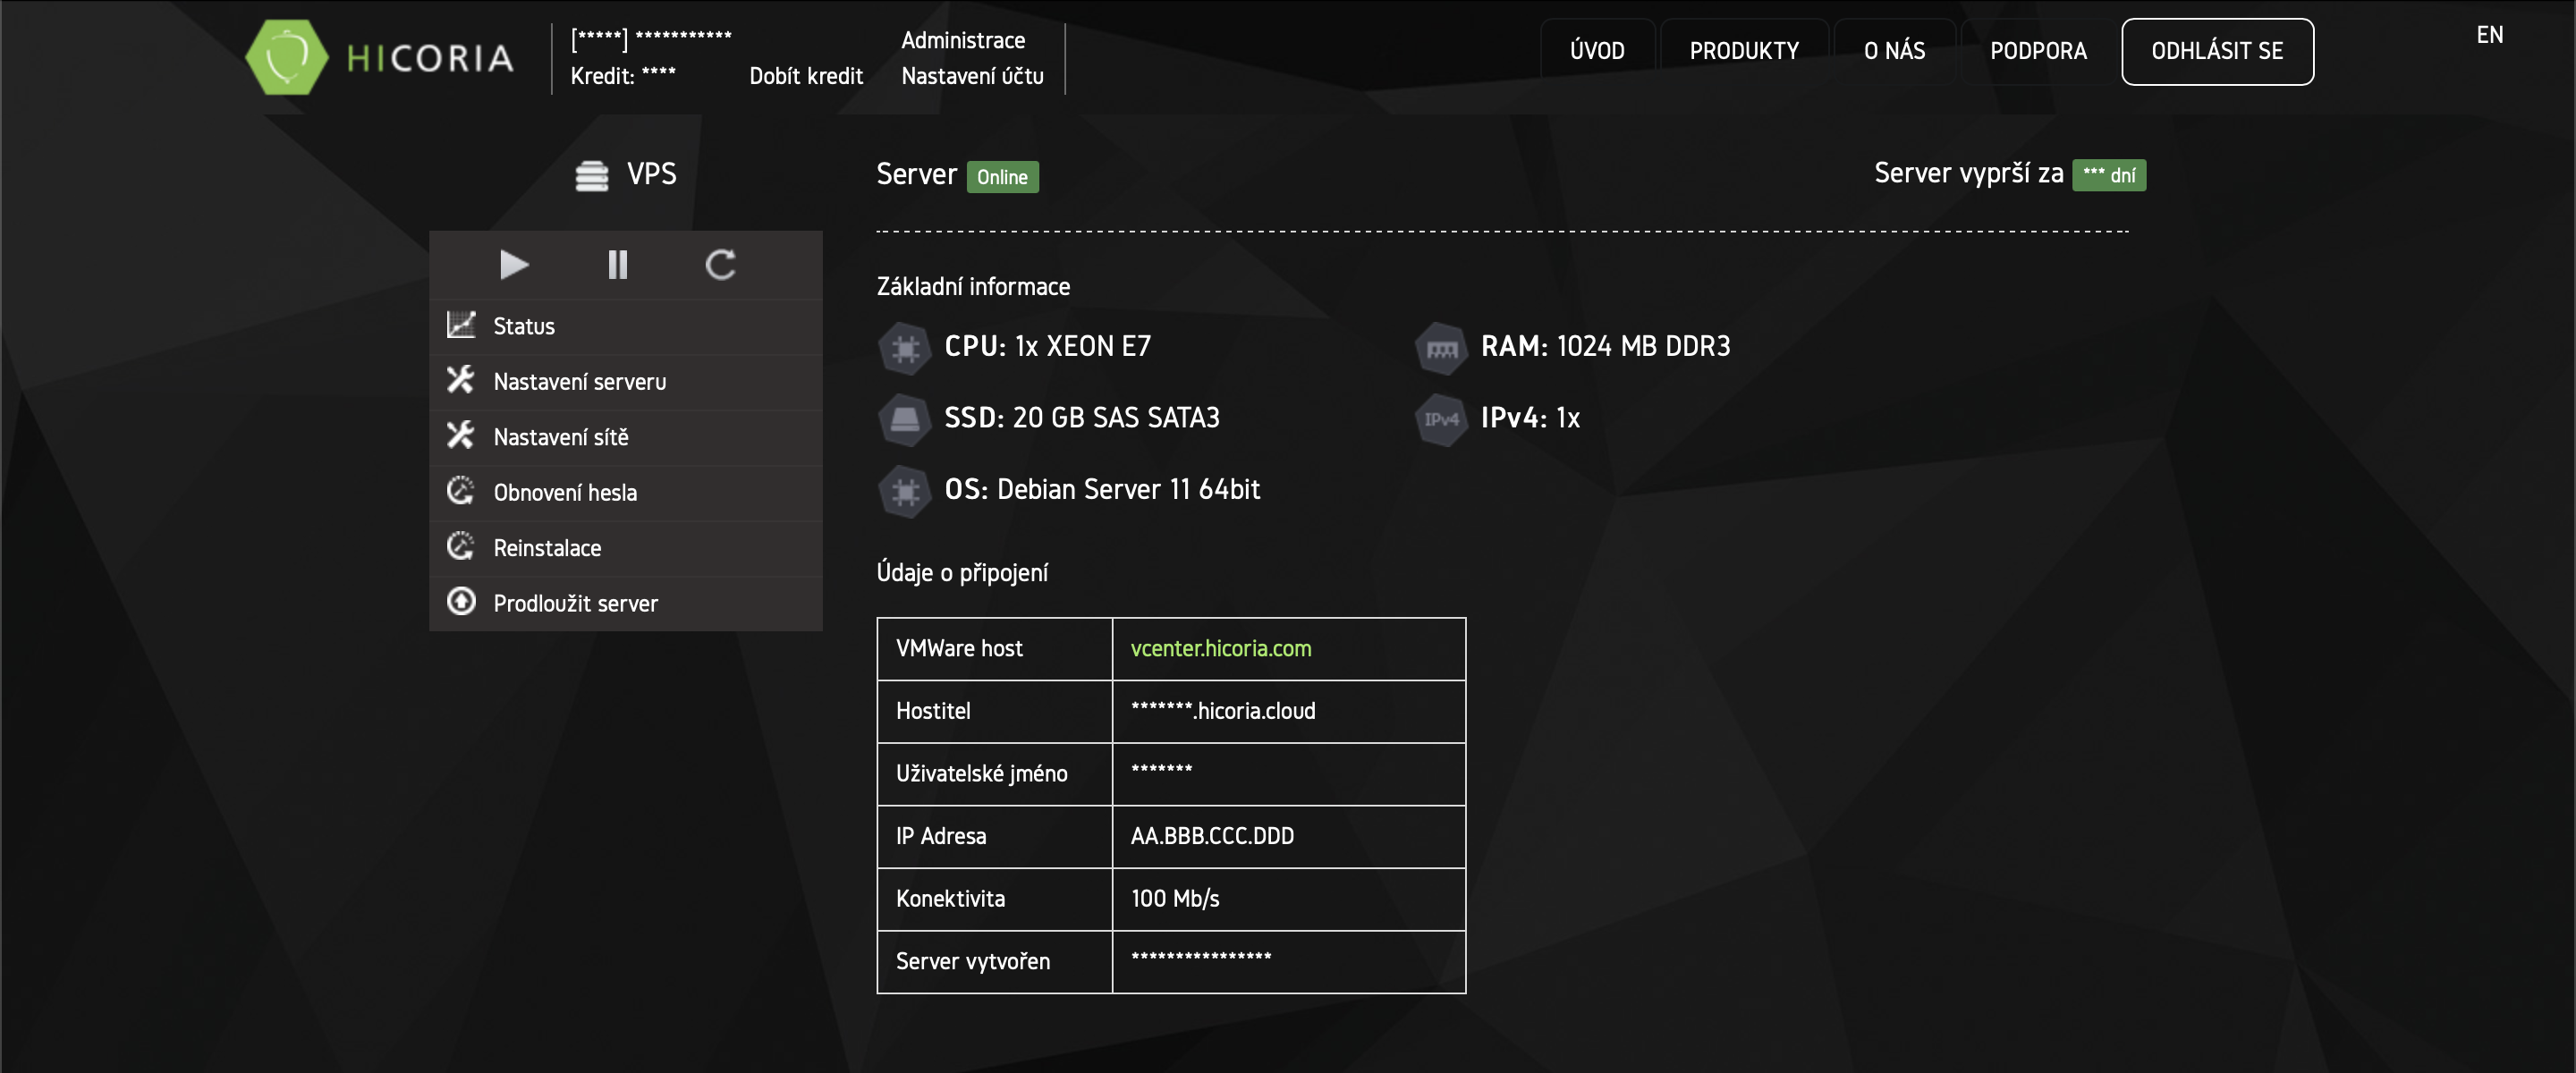
\includegraphics[width=\textwidth]{images/7-nasazeni/7-1-ukazka-hicoria.png}
    \caption{Ukázka administrace virtuálního stroje u společnosti Hicoria}
\end{figure}

Samotné nastavení webového serveru není složité -- stačí nainstalovat Javu, což je s pomocí nástrojů pro Debian jeden příkaz \texttt{sudo apt install default-jdk}. Pro nastavení frameworku Spring Web je následně nutné do konfiguračního souboru \texttt{application.properties} nastavit port, adresu, na které server poběží a také cestu k certifikátu, který bude použit pro HTTPS. Na virtuálním stroji, na který server nasazuji již běží Apache webový server s nastaveným DNS záznamem a HTTPS certifikátem pro doménu \url{https://kvetinac97.cz}, který jsem využil pro účely nasazení API.

\begin{figure}[H]
    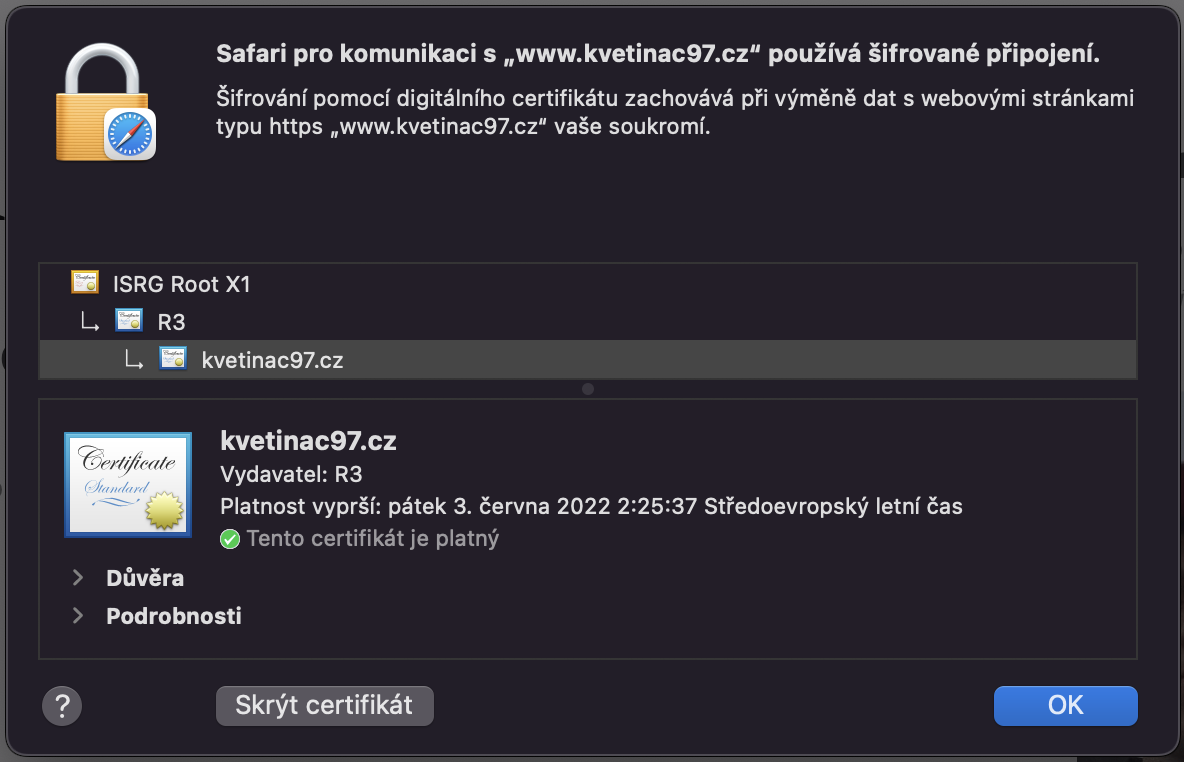
\includegraphics[width=\textwidth]{images/7-nasazeni/7-2-https-server.png}
    \caption[HTTPS certifikát serveru]{HTTPS certifikát serveru na adrese \url{https://kvetinac97.cz}}
\end{figure}

\begin{listing}[H]
\begin{minted}[breaklines,breaksymbolleft=]{properties}
server.port: 8443
security.require-ssl=true
server.ssl.key-store:/etc/letsencrypt/live/kvetinac97.cz/keystore.p12
server.ssl.key-store-password: *****
server.ssl.keyStoreType: PKCS12
server.ssl.keyAlias: *******
\end{minted}
\caption{Konfigurační soubor pro server -- nastavení DNS}
\end{listing}

Aby šlo server spustit, musím zkompilovat kód serveru do spustitelného .jar souboru. Server používá balíčkovací systém Maven \cite{maven}, který obsahuje definici knihoven a závislostí včetně podpůrných knihoven pro Kotlin v konfiguračním souboru \texttt{pom.xml}. Maven obsahuje spustitelný cíl \texttt{mvn package}, který vygeneruje ze zdrojového kódu požadovaný spusitelný soubor ve~formátu jar. Při spuštění serveru je pak důležité server spustit jako systémový proces, aby se po odhlášení uživatele z virtuálního stroje nevypnul, čehož lze jednoduše docílit pomocí POSIX utility \texttt{nohup}. Server je tedy spuštěn příkazem \texttt{nohup java -jar agapesongs.jar \&} a běží na adrese \url{https://kvetinac97.cz:8443}.

\section{App Store}

Jak už jsem psal v kapitole \nameref{testovani}, pro zveřejnění aplikace pro operační systémy iOS a macOS je potřeba tuto aplikaci nahrát do oficiálního obchodu s aplikacemi App Store \cite{app-store}. Stejně jako v případě platformy TestFlight je nejprve potřeba nahrát z programovacího prostředí Xcode verzi aplikace, která musí pro zveřejnění projít schvalovacím procesem App Review. Narozdíl od~TestFlight kontroly je ale tento proces mnohem důkladnější a může se tedy stát, že verze, která projde TestFlight kontrolou, neprojde App Store kontrolou. Po nahrání verze je třeba vyplnit záznam aplikace na platformě App Store Connect \cite{app-store-connect}. Záznam aplikace obsahuje snímky obrazovky, popis a další metadata aplikace. Při kontrole App Review se pak kromě kontroly aplikace samotné kontroluje také záznam v obchodě a jeho soulad s nahranou aplikací.

\begin{figure}
    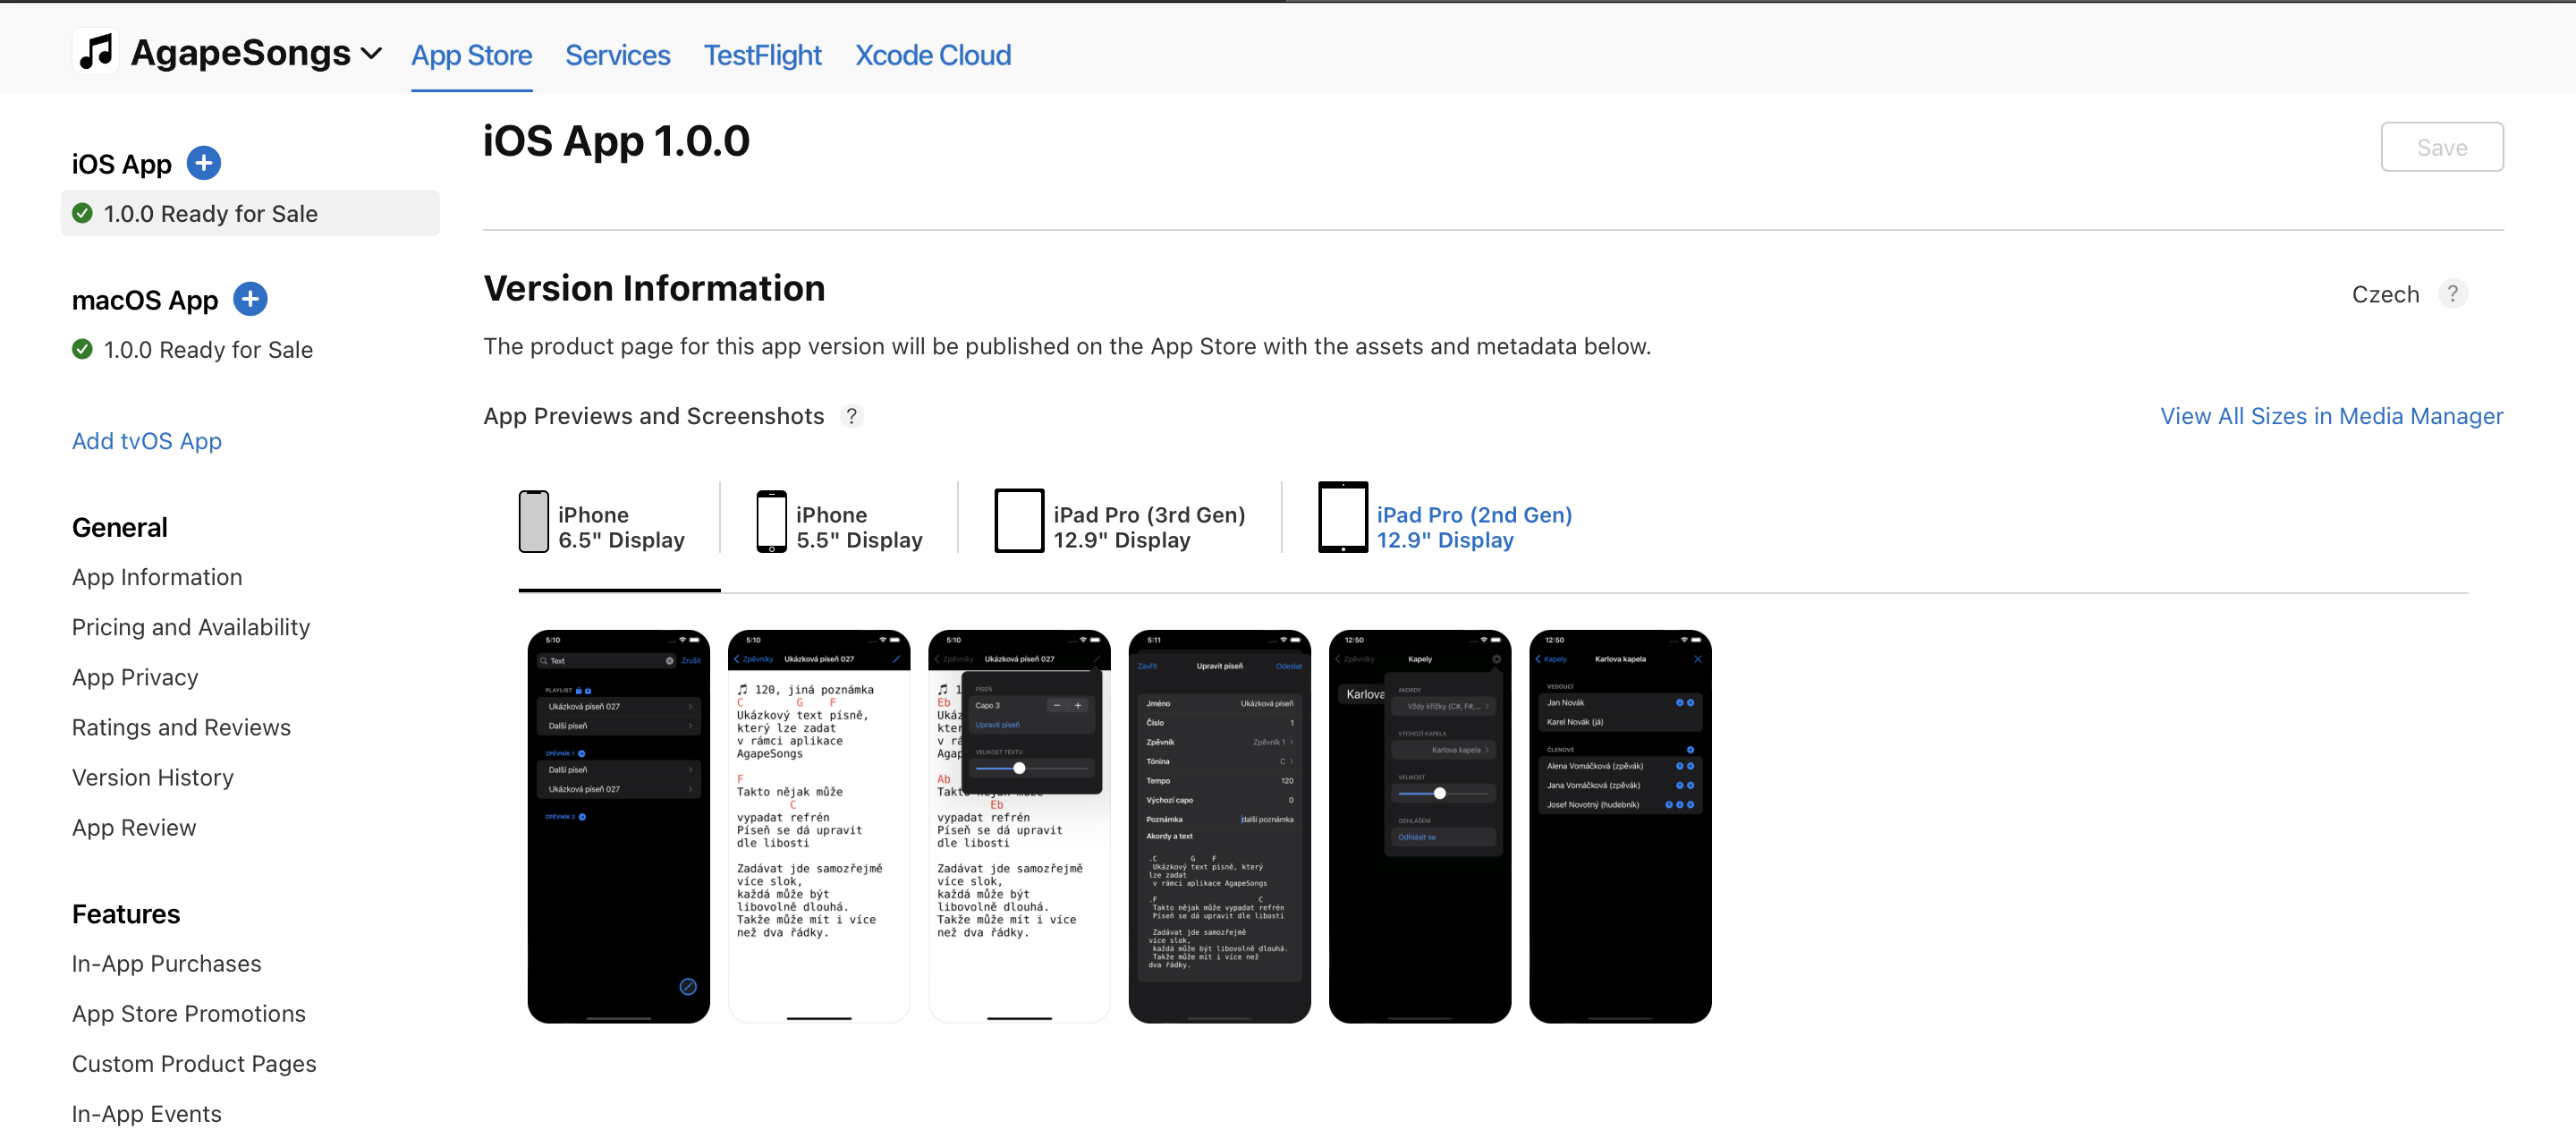
\includegraphics[width=\textwidth]{images/7-nasazeni/7-3-appstore.png}
    \caption{Úvodní obrazovka aplikace v App Store Connect}
\end{figure}

Z vlastních zkušeností z nahrávání aplikací do App Store jsem se pro jistotu rozhodl zkusit nahrát první verzi aplikace už ve čtvrtek 14. 4. 2022. V pátek 15. 4. 2022 mi byla zamítnuta jak iOS, tak macOS verze aplikace. U iOS verze bylo problémem příliš velké tlačítko pro přihlášení přes Apple, což jsem vyřešil změnou jeho velikosti. U macOS bylo problémem označení, že je aplikace serverem (budou se k ní připojovat zařízení ze sítě), i když neumožňuje přijímat příchozí připojení. Toto označení jsem tedy odstranil.

\begin{figure}[H]
    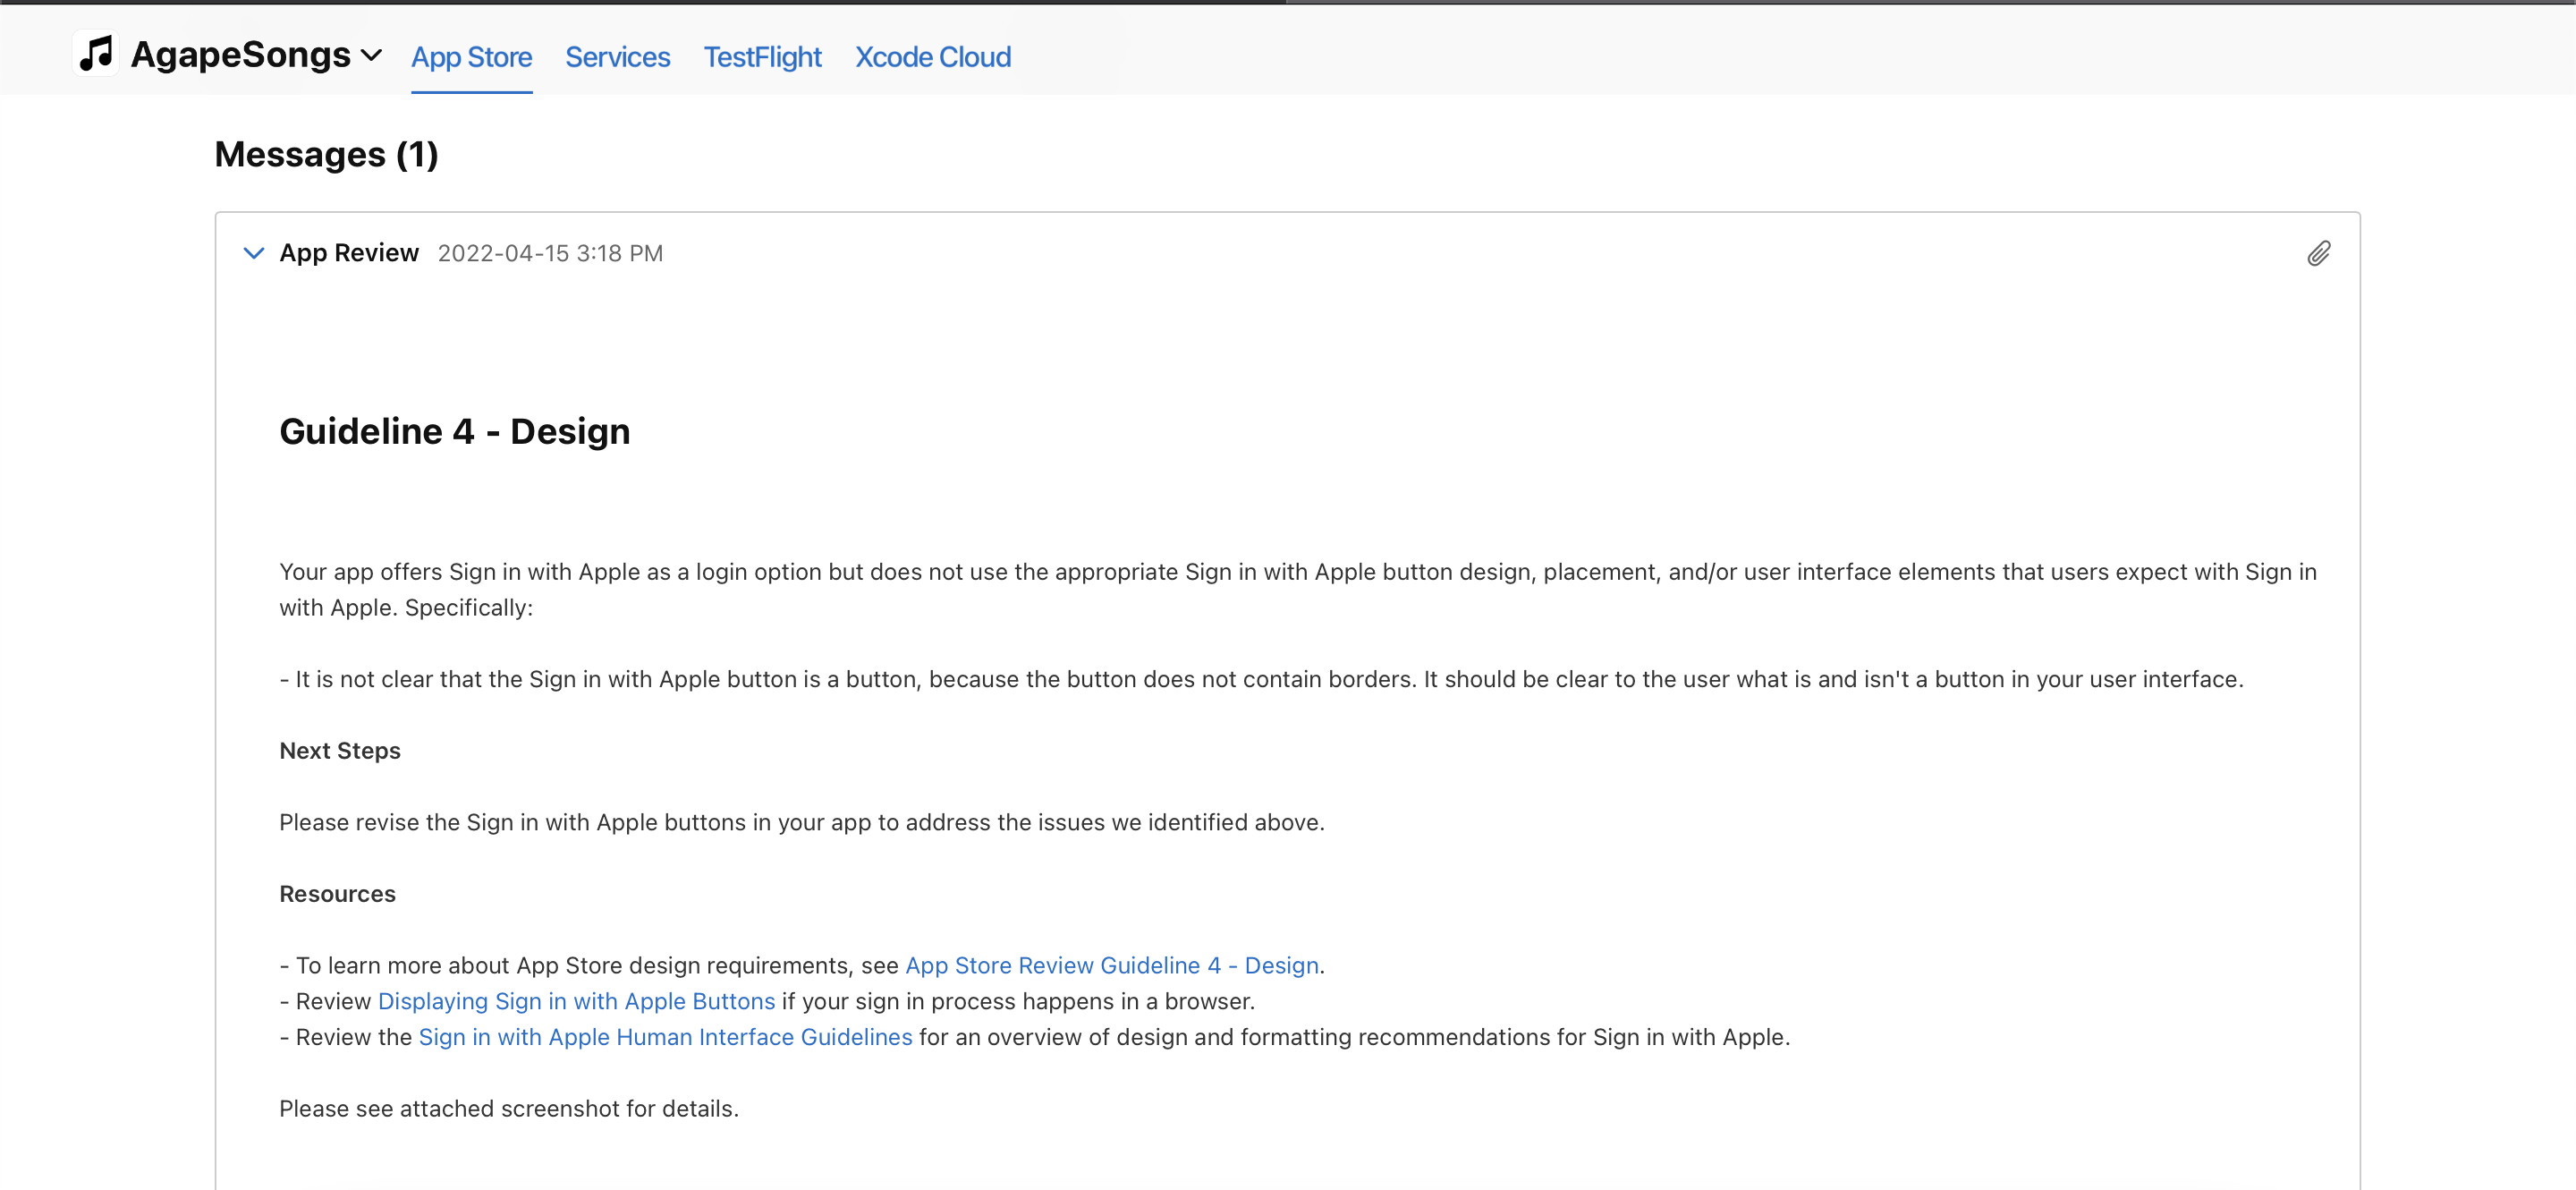
\includegraphics[width=\textwidth]{images/7-nasazeni/7-4-appstore-zamitnuti.png}
    \caption{Informace o zamítnutí aplikace při kontrole App Review}
\end{figure}

Po zmíněných úpravách již aplikace pro obě dvě platformy kontrolou prošly a mohl jsem je vydat veřejně. Jak iOS, tak macOS aplikace jsou tedy veřejně dostupné ke stažení v obchodu pro aplikace App Store.

\begin{figure}[H]
    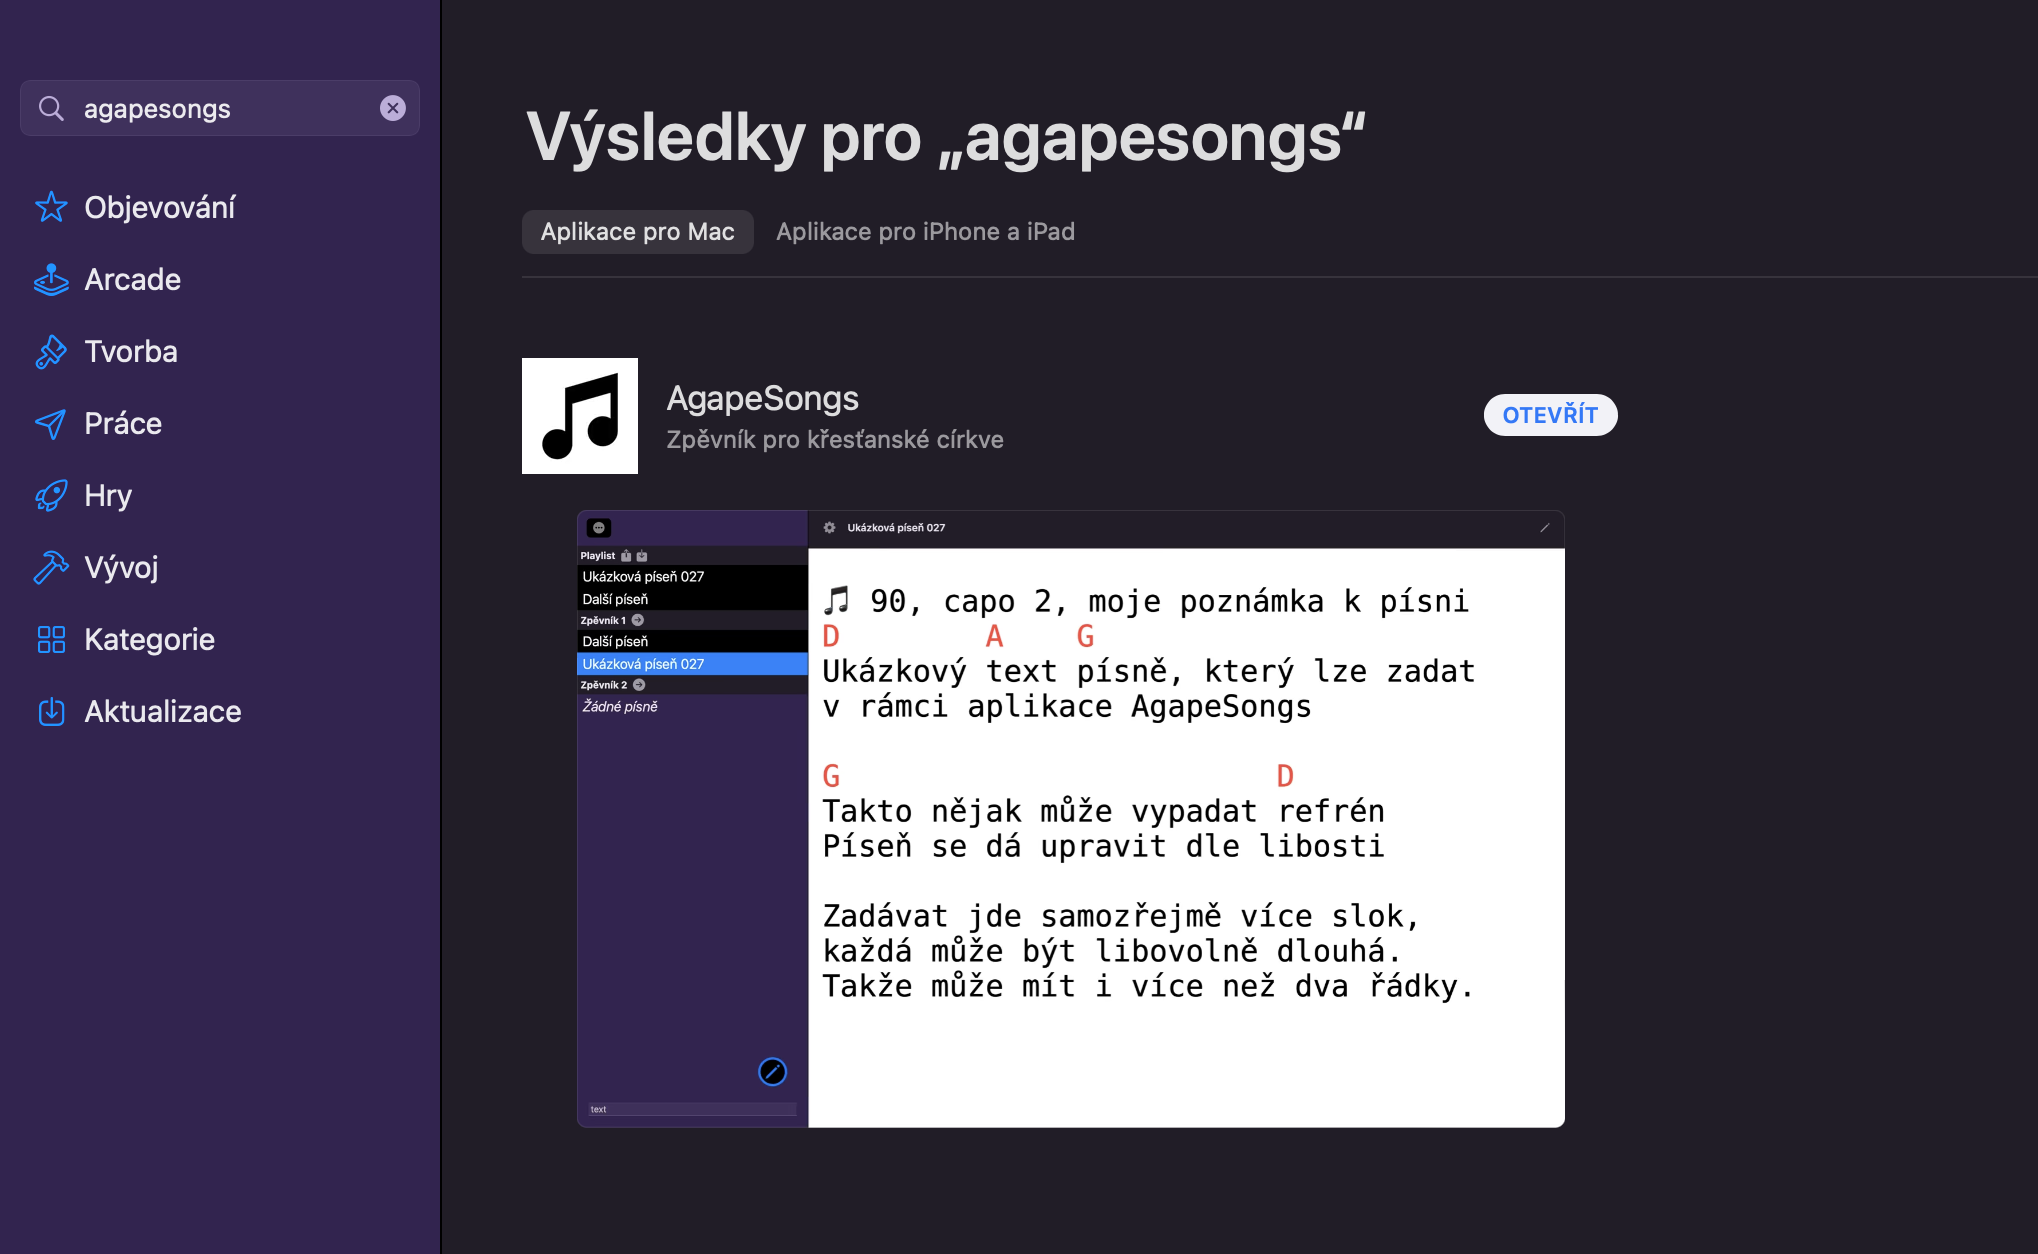
\includegraphics[width=\textwidth]{images/7-nasazeni/7-5-appstore-mac.png}
    \caption{Ukázka aplikace v obchodu pro macOS aplikace App Store}
\end{figure}

\begin{figure}[H]
    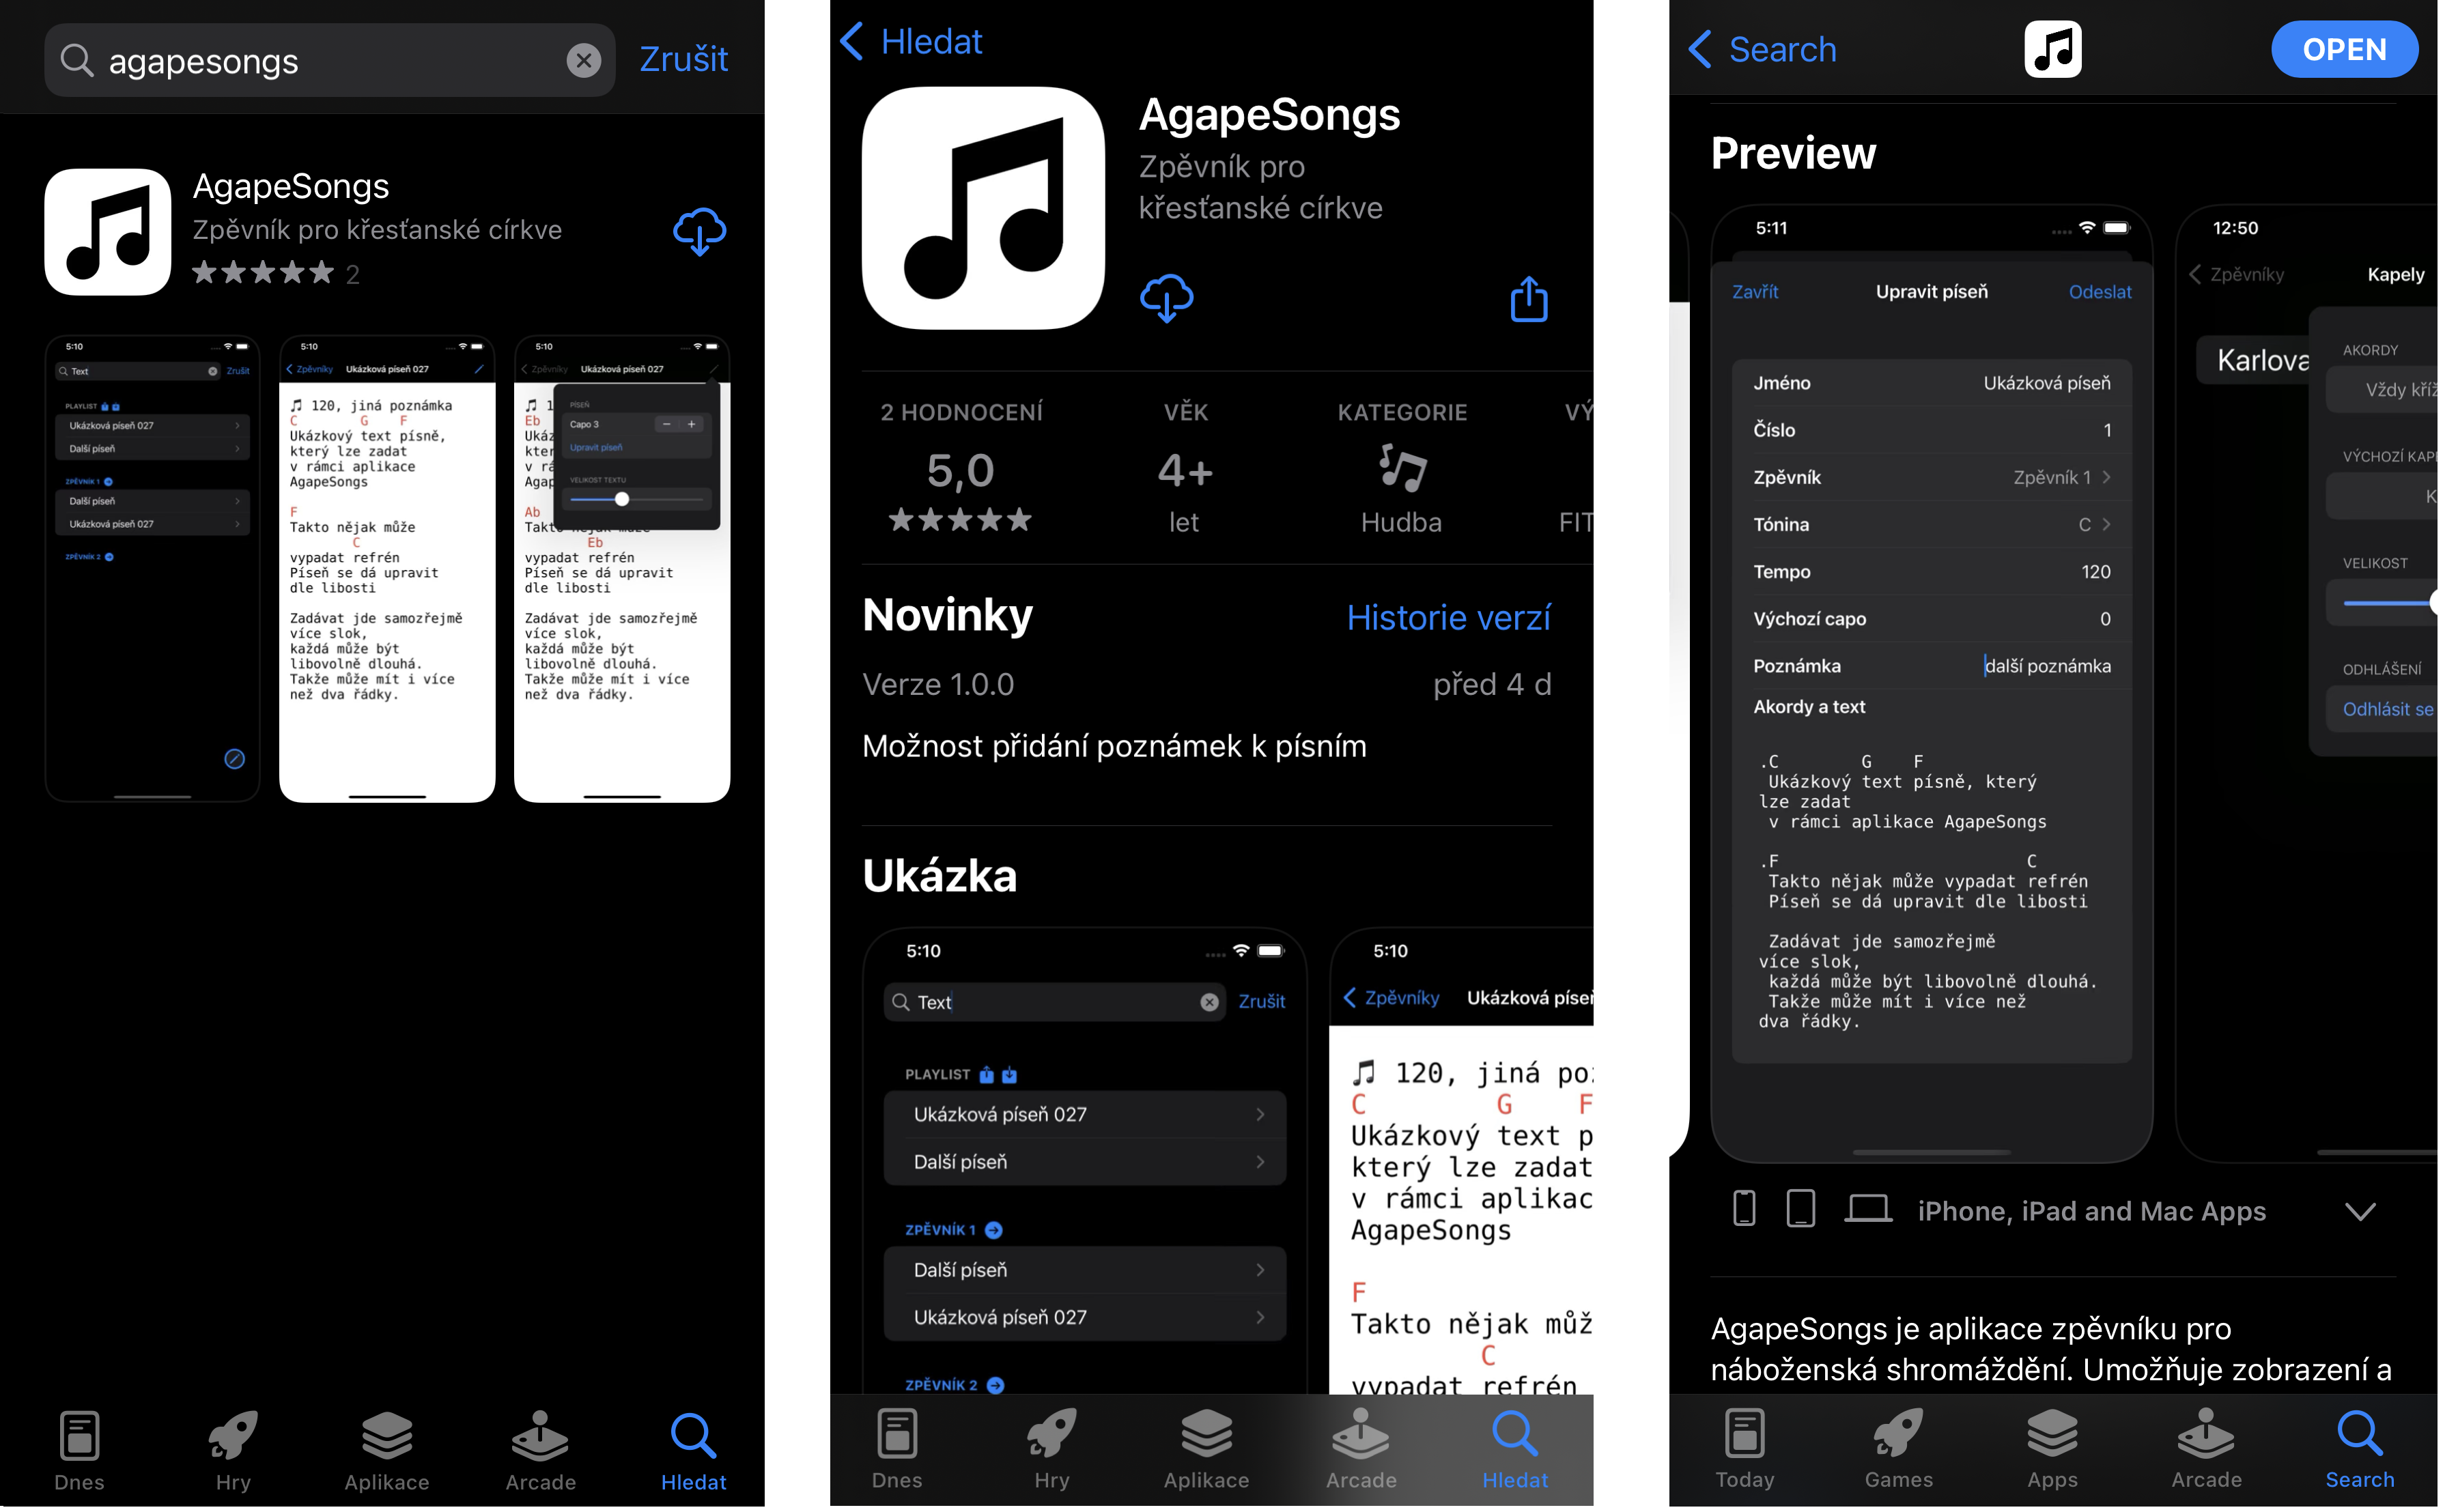
\includegraphics[width=\textwidth]{images/7-nasazeni/7-6-appstore-ios.png}
    \caption{Ukázka aplikace v obchodu pro iOS aplikace App Store}
\end{figure}
